\chapter{Rosaceae}

Here are various plants from the Rosaceae family that I've observed.

\section{Rubus}

There are five species of Rubus that grow near my home:
\begin{itemize}
	\item
	Rubus ursinus: Trailing blackberry
	\item
	Rubus armeniacus: Himalayan blackberry
	\item
	Rubus laciniatus: Cutleaf blackberry
	\item
	Rubus parviflorus: Thimbleberry
	\item
	Rubus spectabilis: Salmonberry
\end{itemize}

\subsection{Rubus ursinus}

\begin{figure}
\centering
\begin{subfigure}{0.47\textwidth}
    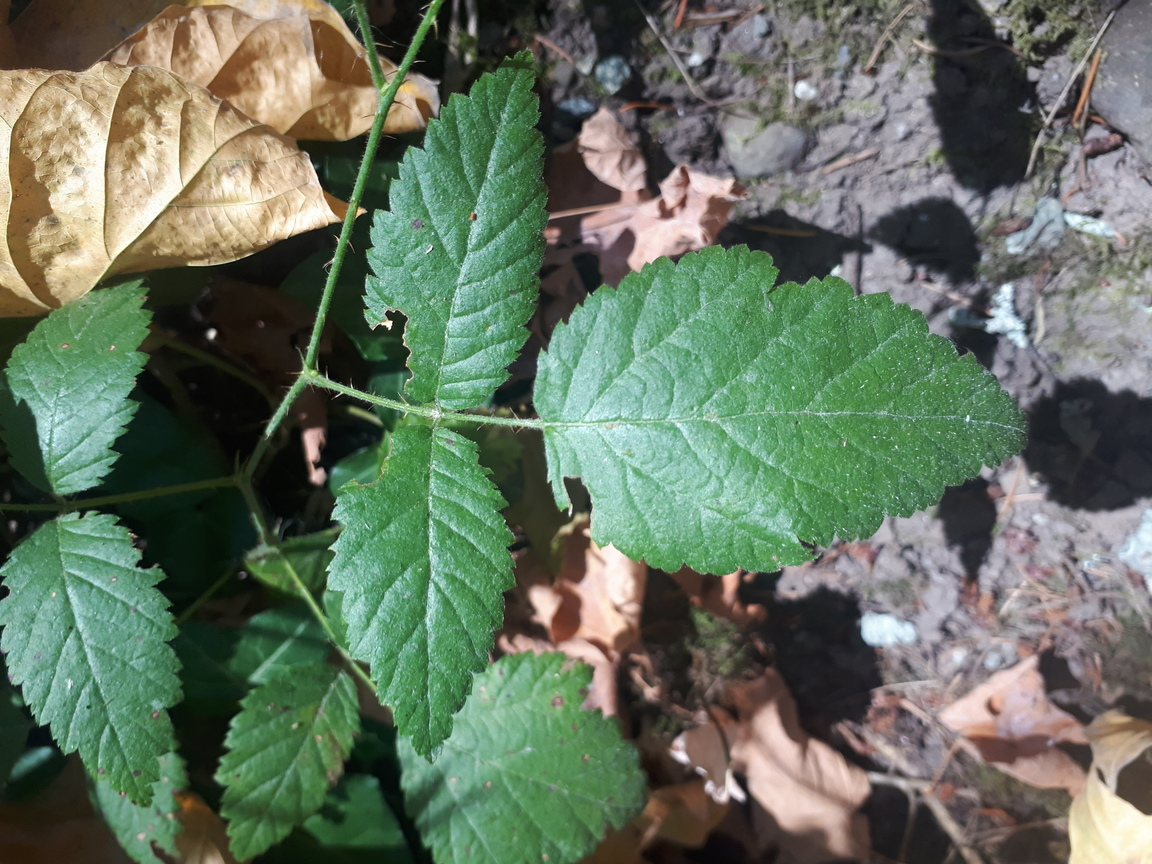
\includegraphics[width=\textwidth]{rubus/ursinus_leaf_01}
    \caption{Leaf}
    \label{fig:rub:ursinus:leaf}
\end{subfigure}
\hfill
\begin{subfigure}{0.47\textwidth}
    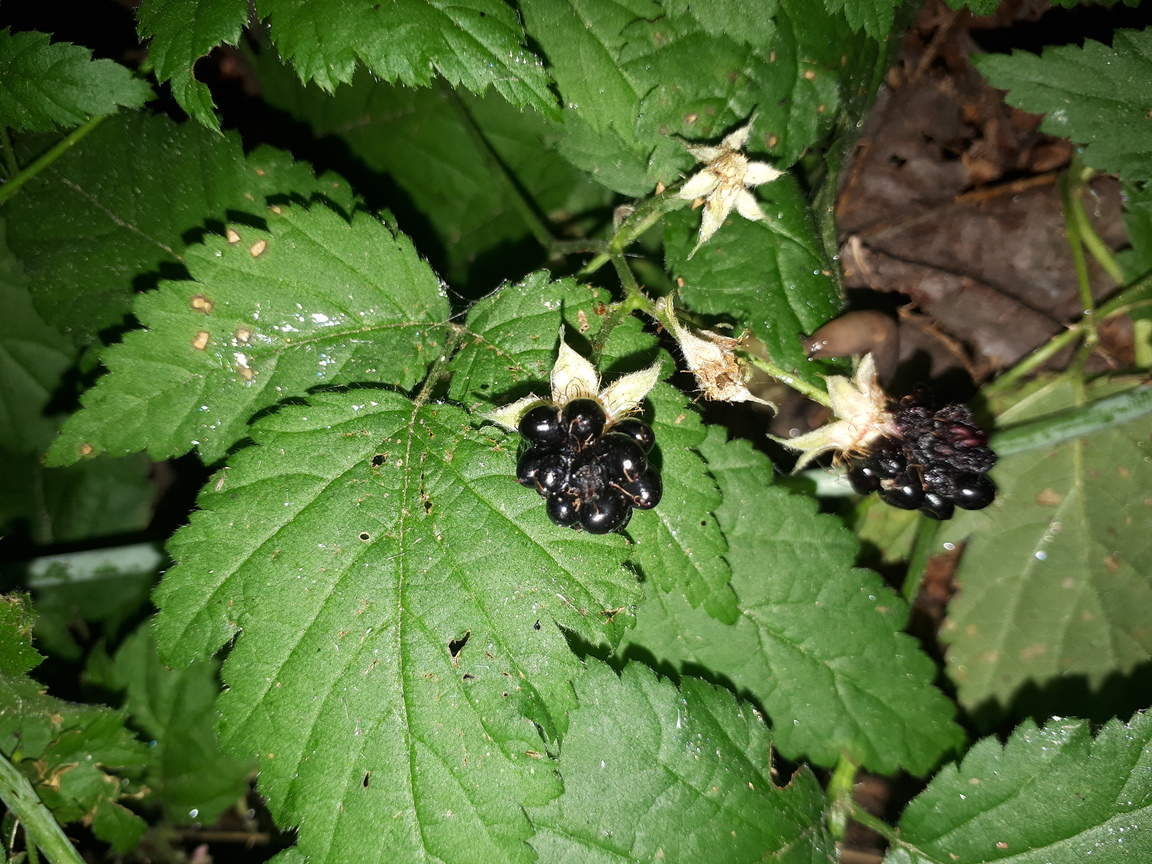
\includegraphics[width=\textwidth]{rubus/ursinus_berry_02}
    \caption{Berry}
    \label{fig:rub:ursinus:berry}
\end{subfigure}
\hfill
\begin{subfigure}{0.47\textwidth}
    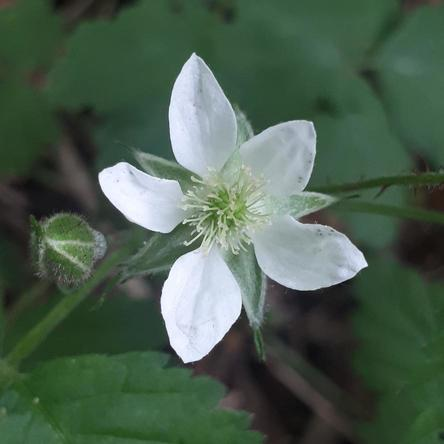
\includegraphics[width=\textwidth]{rubus/ursinus_flower_female_01}
    \caption{Female flower}
    \label{fig:rub:ursinus:flower:female}
\end{subfigure}
\hfill
\begin{subfigure}{0.47\textwidth}
    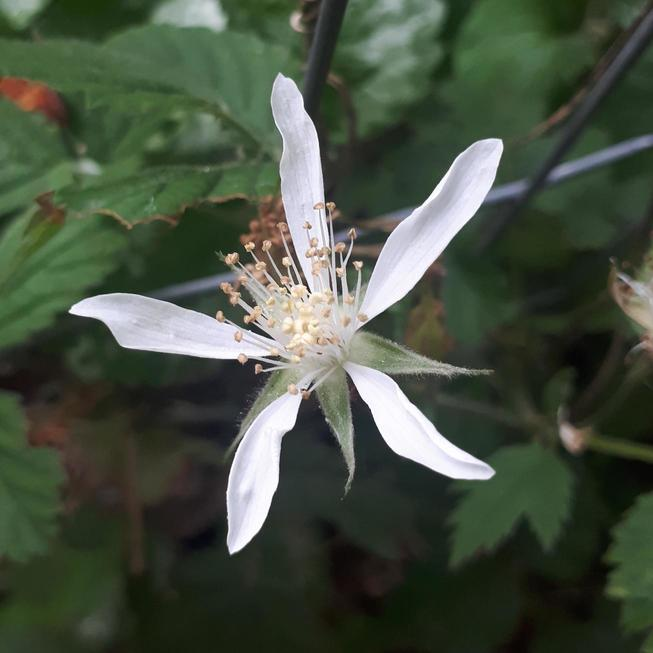
\includegraphics[width=\textwidth]{rubus/ursinus_flower_male_02}
    \caption{Male flower}
    \label{fig:rub:ursinus:flower:male}
\end{subfigure}
        
\caption{Rubus ursinus}
\label{fig:rub:ursinus}
\end{figure}

The trailing blackberry is native to the west coast.

\textbf{Habit:} The plants are low to the ground and crawl along, sending new roots occasionally. The stems are not robust and tend to kinking when manipulated. Stems are covered in fine thorns. I have often found the plants growing under the blankets of English ivy and yellow archangel that cover parts of the yard.

\textbf{The leaves} are compound. Young canes have sets of three, but more mature canes have leaves in sets of five.

\textbf{The canes} are thin with a round cross section. They appear to be coated in a fine powder that gives a blueish green appearance. This power can be rubbed off, revealing green stems. The canes are covered in fine thorns.

\textbf{The flowers} are white. Rubus ursinus has separate male and female flowers, unlike most members of the genus. Male flowers seem to have thinner petals than female flowers.

\textbf{The berries} I've tasted are small and tasty, but not as sweet and juicy as the Himalayan blackberry. When the berry is removed, the receptacle is removed as well. They ripen in early August. 


\newpage

\subsection{Rubus armeniacus}

\begin{figure}
\centering
\begin{subfigure}{0.48\textwidth}
    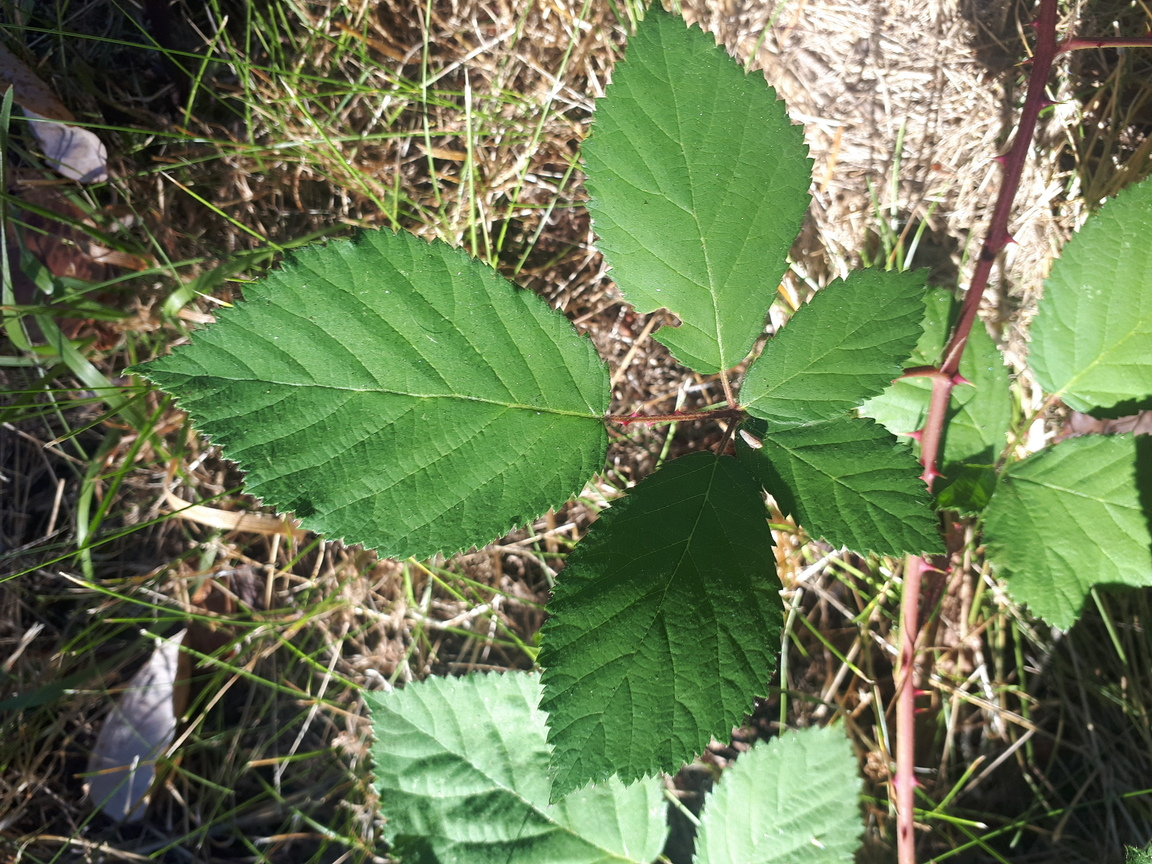
\includegraphics[width=\textwidth]{rubus/armeniacus_leaf_01}
    \caption{Leaf}
    \label{fig:rub:armeniacus:leaf}
\end{subfigure}
\hfill
\begin{subfigure}{0.48\textwidth}
    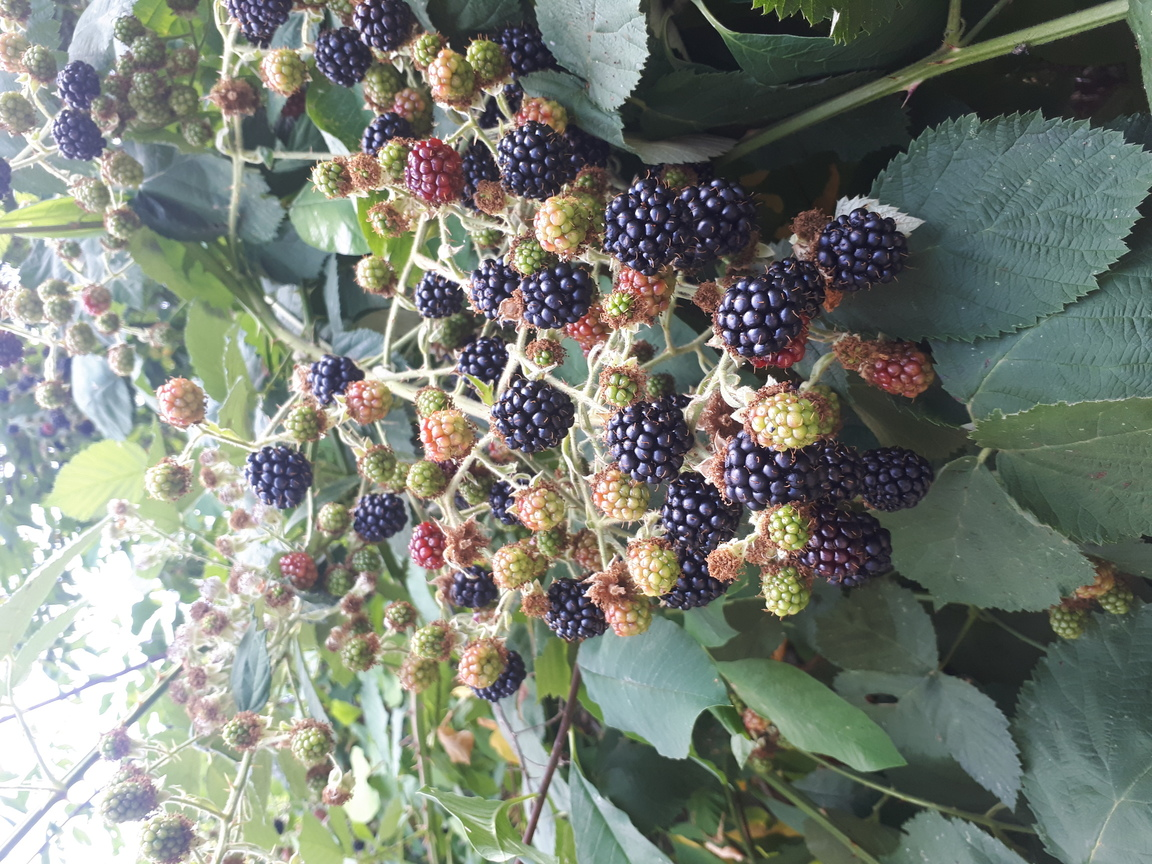
\includegraphics[width=\textwidth]{rubus/armeniacus_berry_01}
    \caption{Berry}
    \label{fig:rub:armeniacus:berry}
\end{subfigure}
\hfill
\begin{subfigure}{0.48\textwidth}
    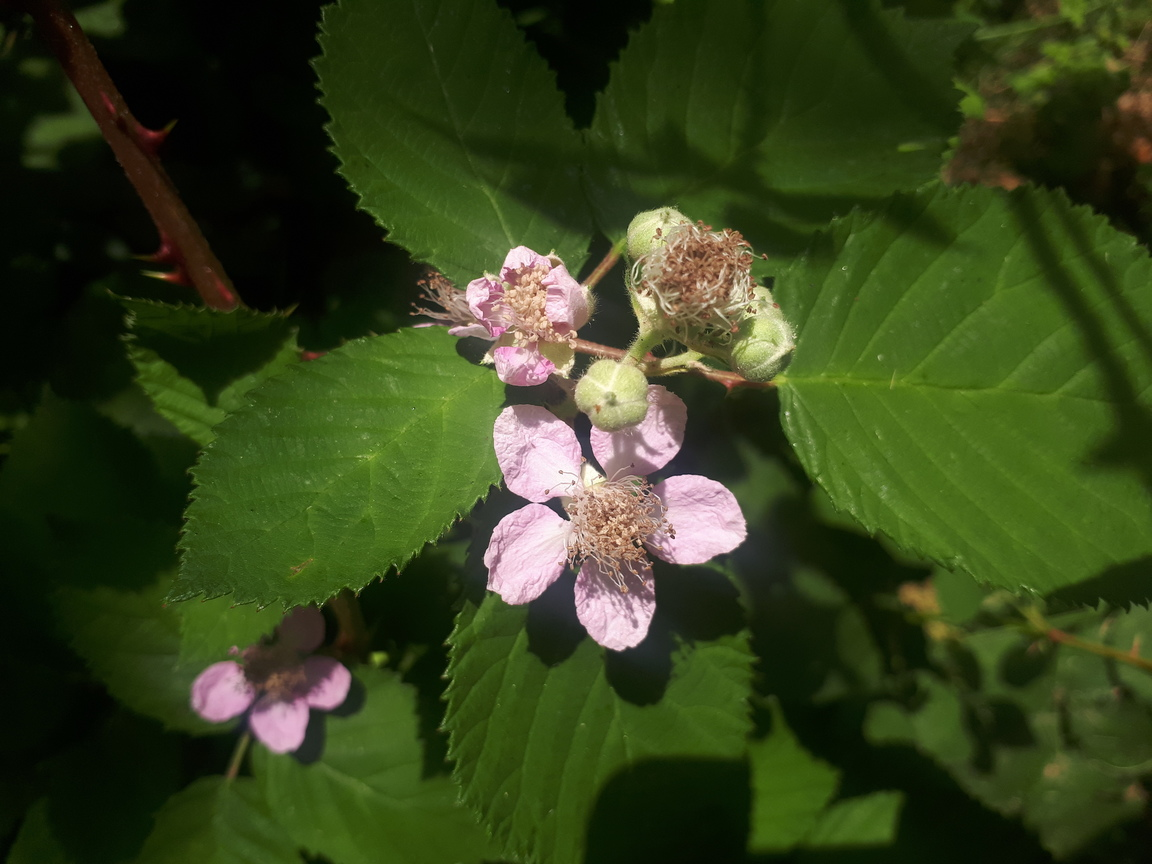
\includegraphics[width=\textwidth]{rubus/armeniacus_flower_01}
    \caption{Flower}
    \label{fig:rub:armeniacus:flower}
\end{subfigure}
\hfill
\begin{subfigure}{0.48\textwidth}
    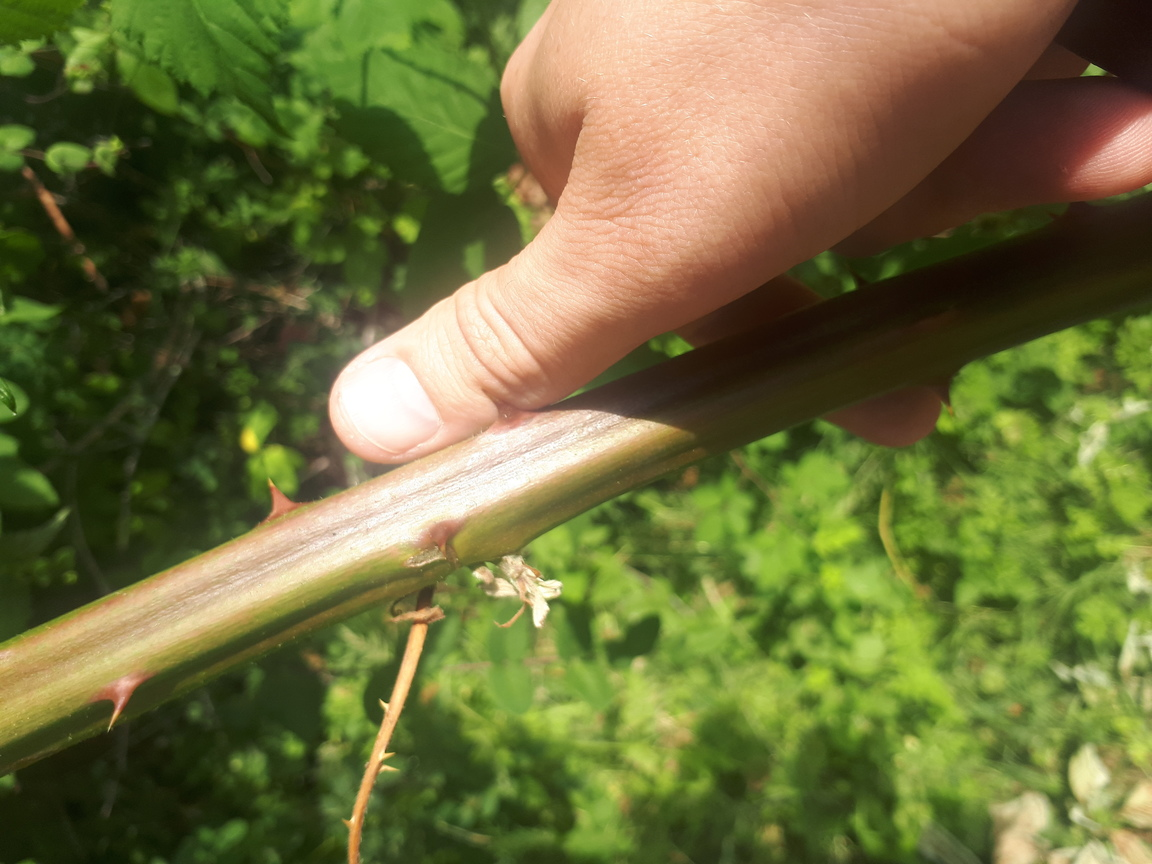
\includegraphics[width=\textwidth]{rubus/armeniacus_cane_01}
    \caption{Cane}
    \label{fig:rub:armeniacus:cane}
\end{subfigure}
        
\caption{Rubus armeniacus}
\label{fig:rub:armeniacus}
\end{figure}

Himalayan blackberry is an invasive species on the west coast and grows anywhere it's not actively removed, such as the side of roads and in empty lots. They are not actually from the Himalayas.

\textbf{Habit:} The plants are erect and produce high arches that get tangled in the foliage of nearby trees. When the arches reach the ground, they may root. Cutting off the branches doesn't stop the plant, as it has a large rootball capable of sending out more shoots. 

\textbf{The leaves} are compound, usually in sets of five. Occasionally the two of the side leaves on a side may be fused into a single leaf with two points. On the branches leading to flowers, the last set of leaves before the flower is generally a set of three.

\textbf{The canes} are robust, 1cm or more in diameter with a pentagonal cross section. They are covered in large thorns. They do not break easily when living. Individual canes are biannual, growing only leaves in the first year, producing flowers and fruit the next year, then dying. The dead stems accumulate, producing a bramble that is difficult to navigate. Dead stems are brittle, with thorns breaking off easily to stick in skin.

\textbf{The flowers} are mostly white with some slight pink. 

\textbf{The berries} are sweet and juicy and very plentiful, ripening in mid August. As with other blackberries, the receptacle is removed with the berry when harvested.



\subsection{Rubus laciniatus}

\begin{figure}
\centering
\begin{subfigure}{0.48\textwidth}
    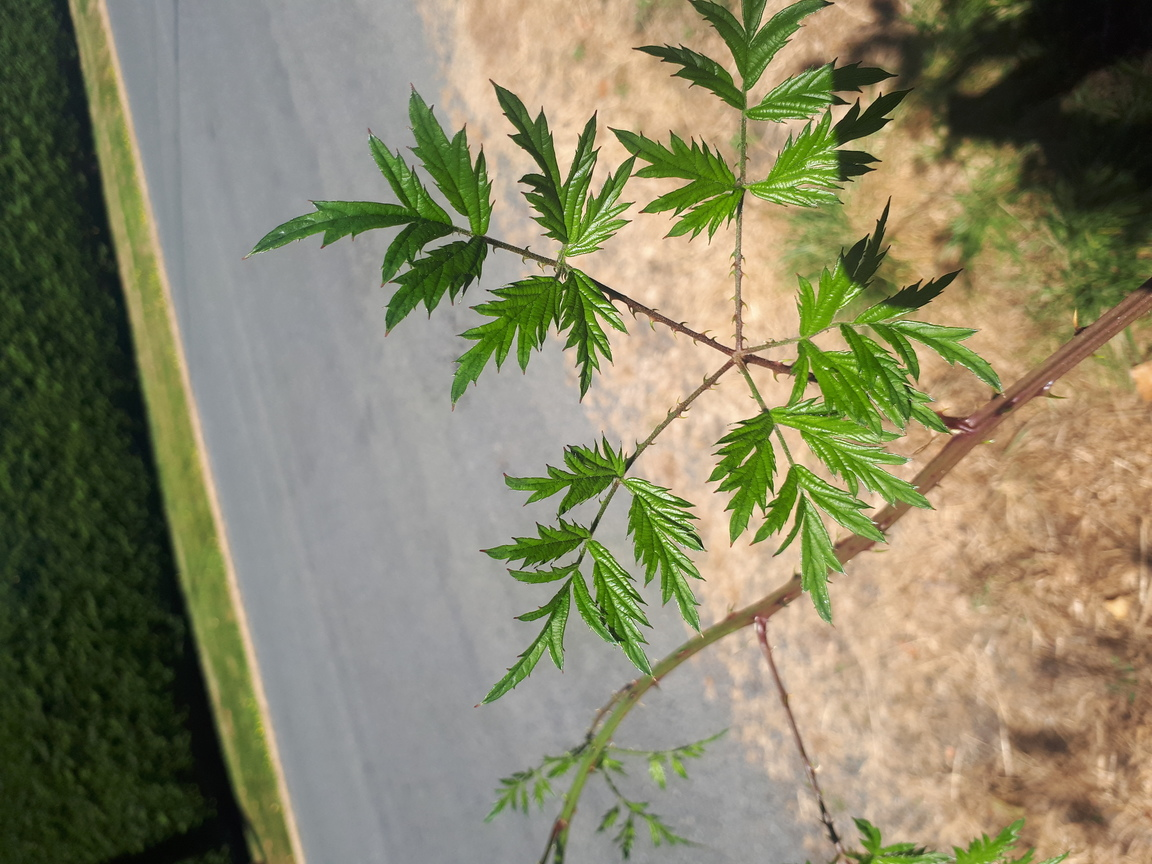
\includegraphics[width=\textwidth]{rubus/laciniatus_leaf_01}
    \caption{Leaf type 1}
    \label{fig:rub:laciniatus:leaf}
\end{subfigure}
\hfill
\begin{subfigure}{0.48\textwidth}
    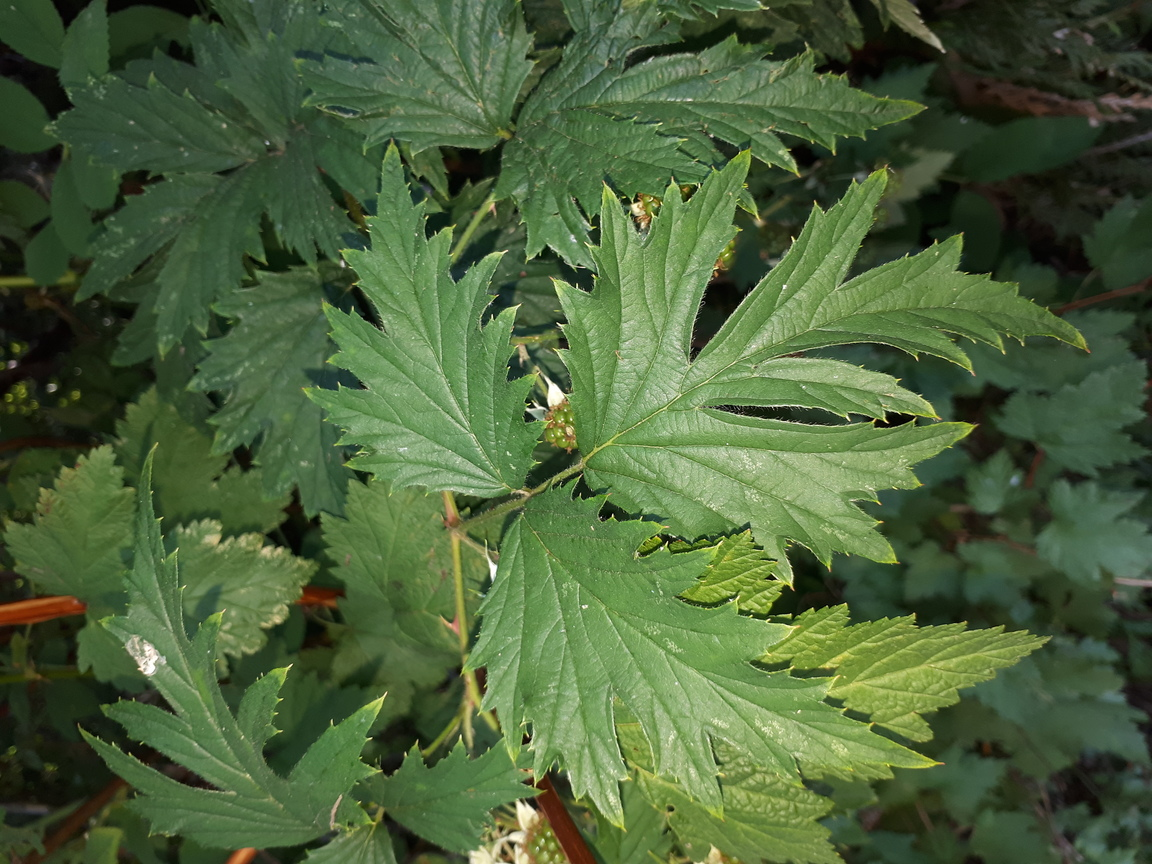
\includegraphics[width=\textwidth]{rubus/laciniatus_leaf_03}
    \caption{Leaf type 2}
    \label{fig:rub:laciniatus:flower}
\end{subfigure}
\hfill
\begin{subfigure}{0.48\textwidth}
    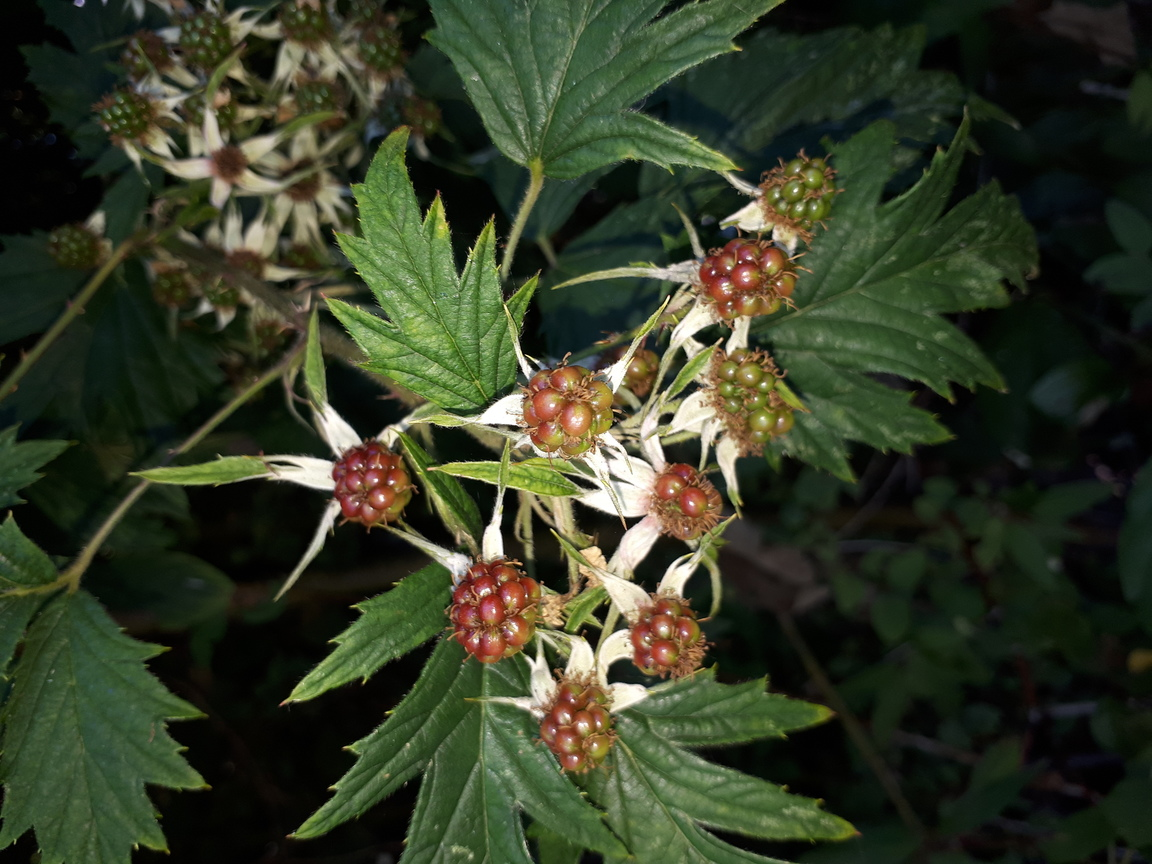
\includegraphics[width=\textwidth]{rubus/laciniatus_berry_01}
    \caption{Berry (unripe)}
    \label{fig:rub:laciniatus:berry}
\end{subfigure}
\caption{Rubus laciniatus}
\label{fig:rub:laciniatus}
\end{figure}

Cutleaf blackberry is also an invasive species, but isn't as widespread as Himalayan blackberry. I have only found it growing in one place.

\textbf{Habit:} Similar to Himalayan blackberry as far as I can tell.

\textbf{The leaves} are compound in sets of five, with each leaflet also divided into a set of five. The leaves near the flowers are generally in sets of three, with much less subdivision than the main stem leaves.

\textbf{The canes} are similar to Himalayan blackberry, also having pentagonal cross sections. The thorns on this species seem to be especially sharp.

\textbf{The flowers} have not been observed by me.

\textbf{The berries} taste similar to Himalayan blackberry. As with other blackberries, the receptacle comes off when the berry is picked


\subsection{Rubus parviflorus}

\begin{figure}
\centering
\begin{subfigure}{0.48\textwidth}
    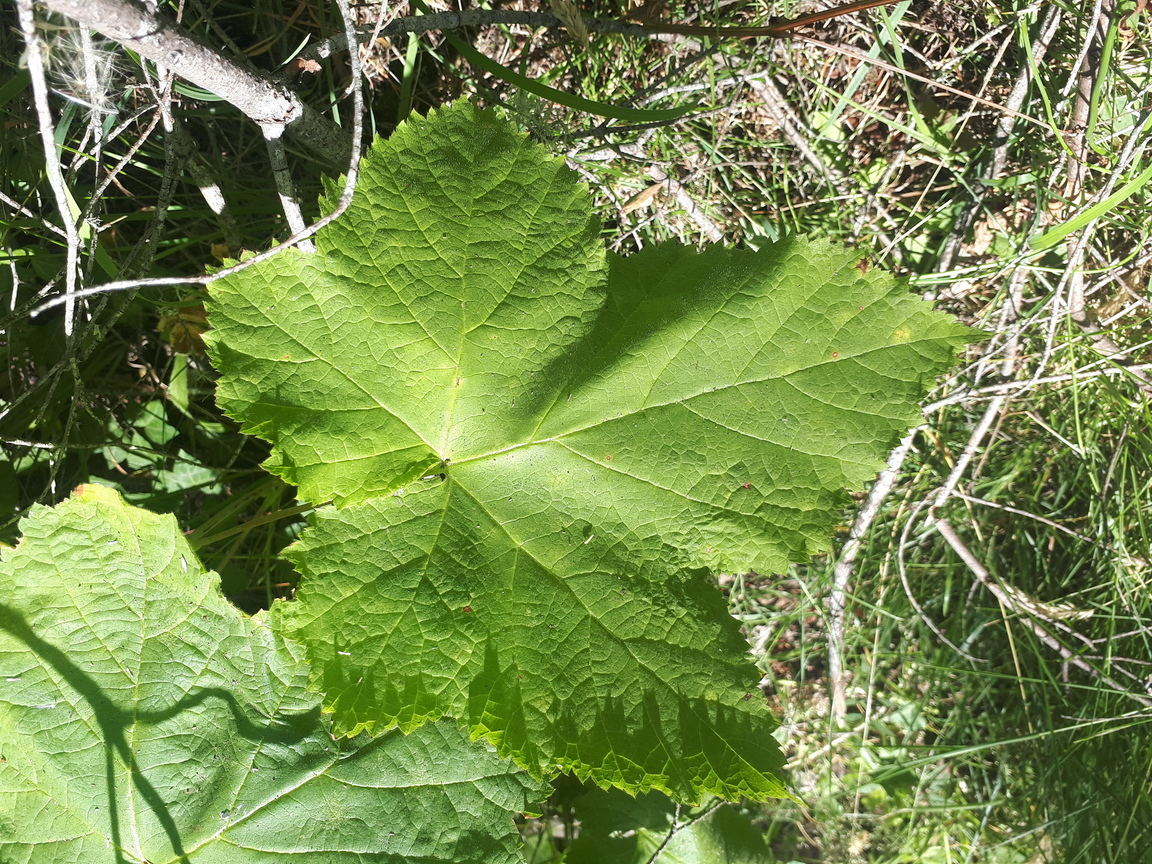
\includegraphics[width=\textwidth]{rubus/parviflorus_leaf_01}
    \caption{Leaf}
    \label{fig:rub:parviflorus:leaf}
\end{subfigure}
\hfill
\begin{subfigure}{0.48\textwidth}
    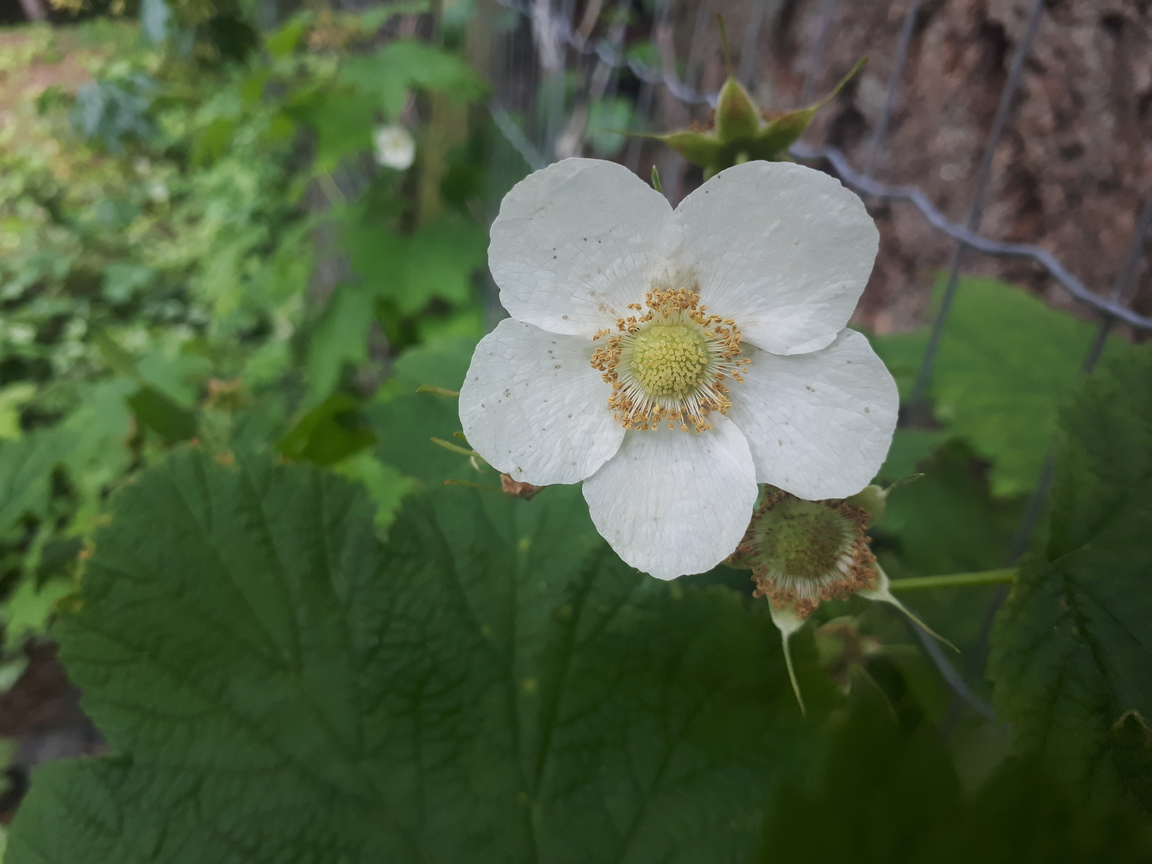
\includegraphics[width=\textwidth]{rubus/parviflorus_flower_01}
    \caption{Flower}
    \label{fig:rub:parviflorus:flower}
\end{subfigure}
\hfill
\begin{subfigure}{0.48\textwidth}
    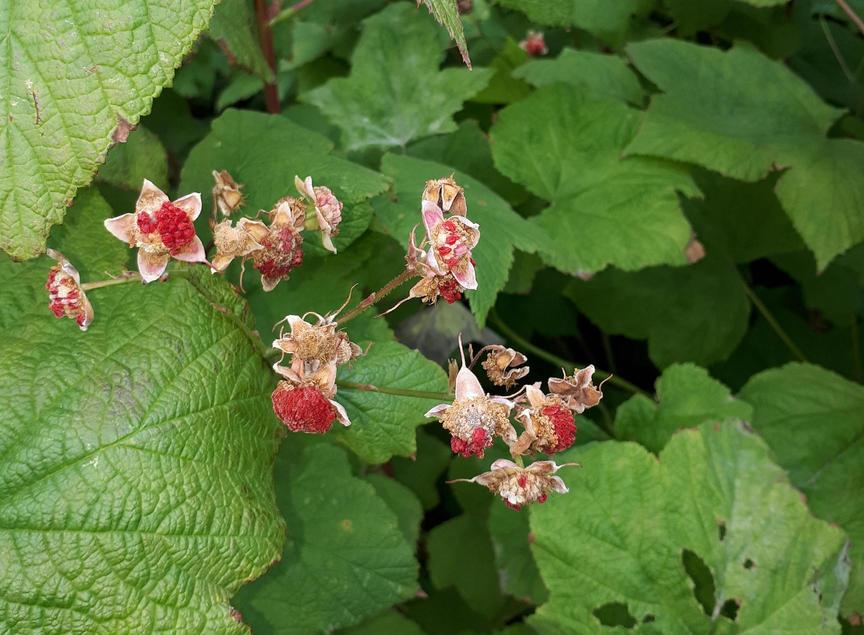
\includegraphics[width=\textwidth]{rubus/parviflorus_berry_01}
    \caption{Berry}
    \label{fig:rub:parviflorus:berry}
\end{subfigure}

        
\caption{Rubus parviflorus}
\label{fig:rub:parviflorus}
\end{figure}

Thimbleberry is native to the west coast. The name `parviflorus' means small-flowered, despite the flowers of this species being especially large for its genus

\textbf{Habit:} The plant has a shrublike habit, growing about four feet tall. 

\textbf{The leaves} are large and simple, shaped similar to maples with five lobes. Unlike the many other Rubus species, the individual leaflets have fused into a single leaf. Leaves closest to flower/berries seem to only have three lobes, which matches the general pattern I've seen in this genus. The leaves have a fine soft hair

\textbf{The canes} are thin, with no thorns.

\textbf{The flowers} are white and relatively large with round petals.

\textbf{The berries} are small and bright red, coming off the plant like a thimble with the receptacle left behind. They are sweet and grainy, not particularly juicy. The individual `bits' of the berry are small relative to other rubus berries. I have not found the plants to be very productive with berries the way blackberries tend to be.


\subsection{Rubus spectabilis}

\begin{figure}
\centering
\begin{subfigure}{0.48\textwidth}
    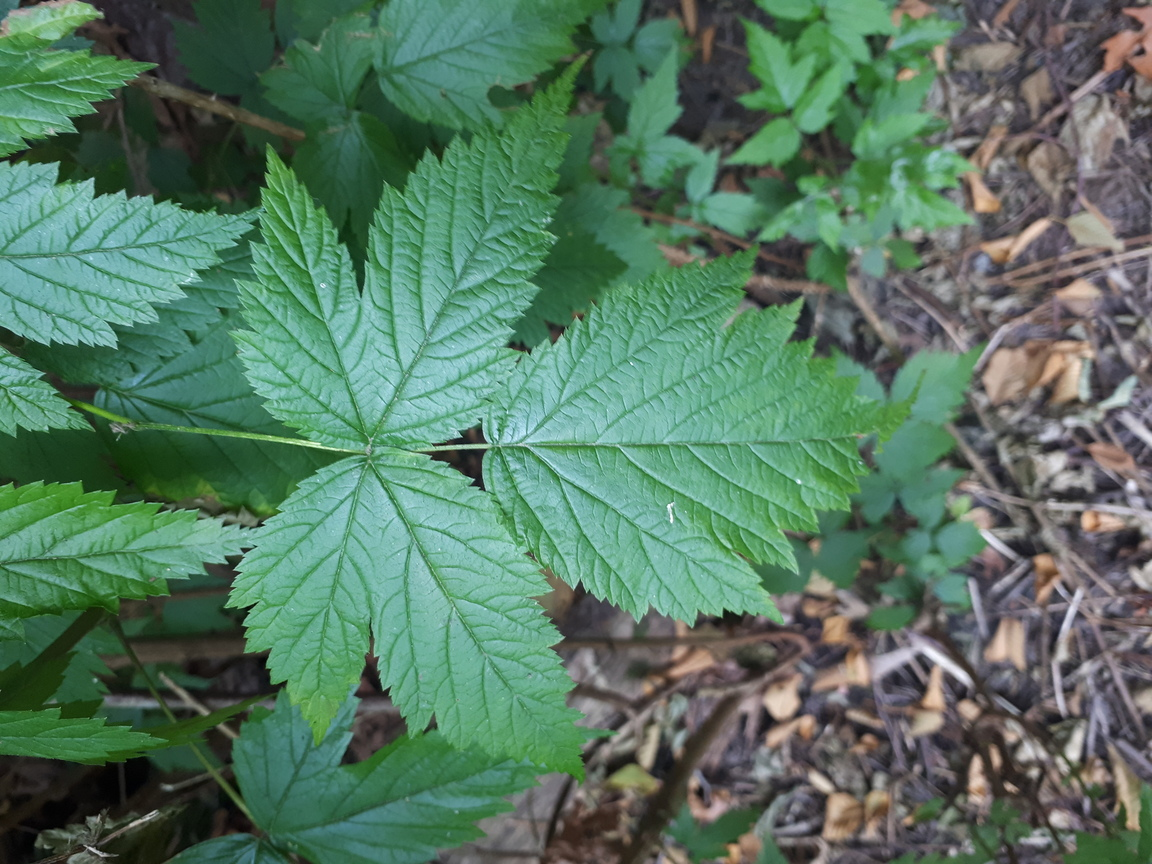
\includegraphics[width=\textwidth]{rubus/spectabilis_leaf_01}
    \caption{Leaf}
    \label{fig:rub:spectabilis:leaf}
\end{subfigure}
\hfill
\begin{subfigure}{0.48\textwidth}
    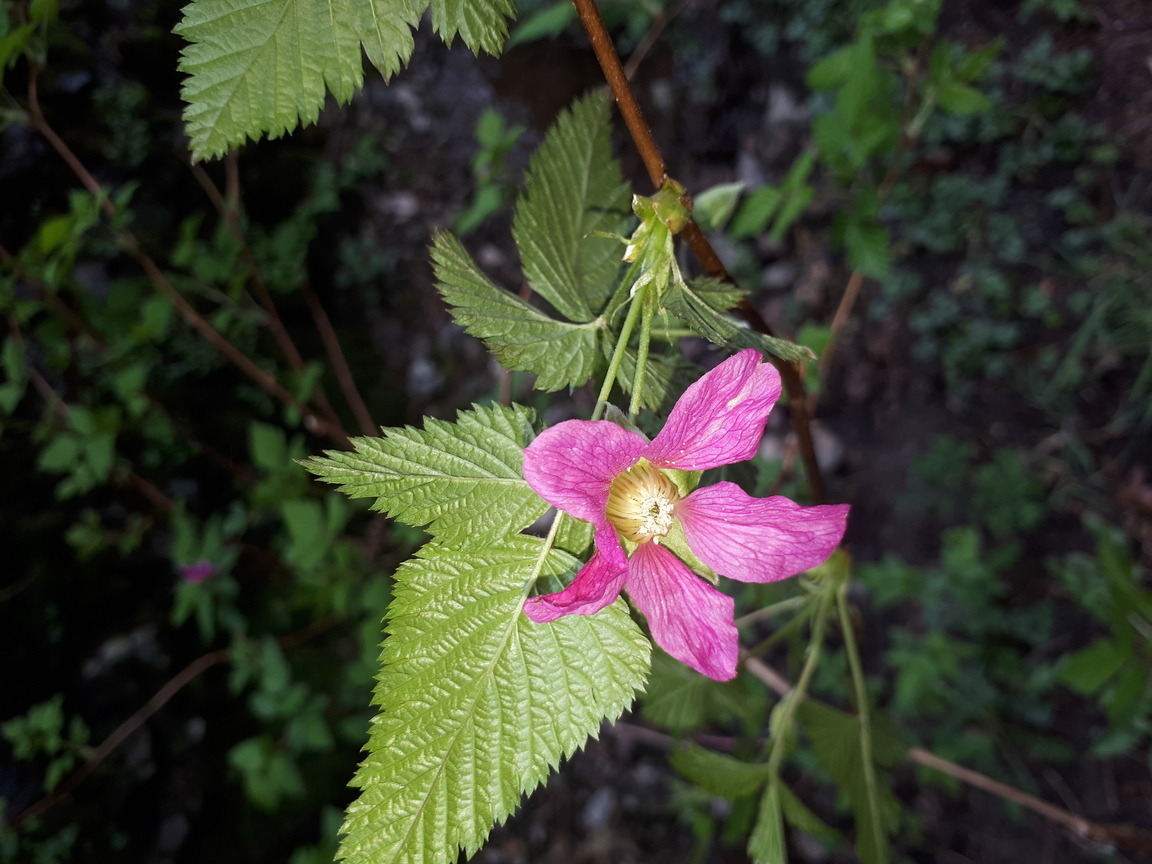
\includegraphics[width=\textwidth]{rubus/spectabilis_flower_01}
    \caption{Flower}
    \label{fig:rub:spectabilis:berry}
\end{subfigure}

        
\caption{Rubus spectabilis}
\label{fig:rub:spectabilis}
\end{figure}

Salmonberry is native to the west coast.

\textbf{Habit:} The plants have a more tree like habit, growing quite tall with woody stems.

\textbf{The leaves} are compound sets of three, with the lower leaves having two lobes like fusion of the side leaves of a Himalayan blackberry. The leaves closest to the flower lack these second lobes.

\textbf{The canes} are woody and perennial, with sparse thorns.

\textbf{The flowers} are dark pink.

\textbf{The berries} are large and pink-orange, similar in colour to salmon flesh. They are juicy and mild tasting and ripen in early summer.


\section{Acer}

Bigleaf maple

\section{Rosa}

Nootka rose

